\section{Introduction}

\frame{
	\frametitle{The Project}

	\begin{itemize}
  		\item The vision of a human being will be expanded by information about the environment
		\item The information that will displayed is, if a classrooms status is occupied or free.
		\item Uses QR-codes, which are sticked to the classrooms entrance.
		\item Scanning this code using the Vuzix M100. 
		\item An image will be projected on the plate and indicates whether the classroom is occupied in the next lesson or free.
	\end{itemize}
	
	\begin{block}{Projections}
		\begin{center}
	    	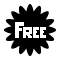
\includegraphics[width=15mm]{content/figures/free}
	    	\hspace{30mm}
		    
\includegraphics[width=15mm]{content/figures/stop}
		\end{center}
	\end{block}
}

\subsection{Technologies}
\frame{
	\frametitle{Technologies}
	
	\begin{itemize}
		\item Vuzix Smart Glasses M100 with Flash Image v2.4.3
		\item Android is the OS.
		\item Built-in 'Scanner' App for QR-Code scanning.
		\item OpenGL ES to project the two images.
	\end{itemize}
}

\subsection{Architecture}
\frame{
	\frametitle{Architecture}
	
	\begin{itemize}
		\item MainActivity, which …
		\item Using a built-in 'Scanner' App.
		\item RenderActivity, which …
		\item OpenGL Elements, which draws/projects the images.
		\item TableReader, which loads the room informations.
	\end{itemize}	
}